%%%%%%%%%%%%%%%%%%%%%%%%%%%%%%%%%%%%%%%%%%%%%%%%%%%%%%%%%%%%%%%%%%%%%%%%%%%%%%%%%%%
%% Software Engineering: Project Management
%% CMMI: Project Monitoring and Control
%%
%% Yannick Drost, Tobias Stoll, Dominik Schreiber
%% winter term 2012/2013, TU Darmstadt
%%%%%%%%%%%%%%%%%%%%%%%%%%%%%%%%%%%%%%%%%%%%%%%%%%%%%%%%%%%%%%%%%%%%%%%%%%%%%%%%%%%
\documentclass[accentcolor=tud1b]{tudbeamer}

% ===== Packages ==================================================================
\usepackage[utf8]{inputenc}
\usepackage[ngerman]{babel}
\usepackage[T1]{fontenc}

\usepackage{color}
\usepackage{listings}
\usepackage{multicol}
%\usepackage[sectionbib]{natbib}
%\usepackage{chapterbib}

% ===== Commands, Changes =========================================================
\newcommand{\strong}[1]{\textaccentcolor{\textsf{\textbf{#1}}}}

% ----- shorthand for creating a frame with current headline+subheadline ----------
\newcount\Level
\let\Part=\part\def\part{\global\Level=0\Part}
\let\Chapter=\chapter\def\chapter{\global\Level=1\Chapter}
\let\Section=\section\def\section{\global\Level=2\Section}
\let\Subsection=\subsection\def\subsection{\global\Level=3\Subsection}
\let\Subsubsection=\subsubsection\def\subsubsection{\global\Level=4\Subsubsection}

% creates a frame with a frametitle of up to two lines, depending on the current
% document structure. that means: 
% 	- if the tframe is created inside a section, it will have the sections header
% 	  as frametitle
% 	- if the tframe is created inside a subsection, it will have the sections
% 	  header as frametitle followed by the subsections header in the next line
% 	- if the tframe is created inside a subsubsection, it will have the subsections
% 	  header as frametitle followed by the subsubsections header in the next line
% each frametitle can be additionally adjusted by the optional argument. any text
% in there will be printed as \textnormal and appended to the second line with one
% space between the content and the appended text.
%
% usage:
% 	\begin{tframe}[optional addition to the subtitle]
% 		use it just as any normal frame
% 	\end{tframe}
\newenvironment*{tframe}[1][]{%
	\begin{frame}
	\ifnum\Level=2
		\frametitle{\insertsectionhead\\\strong{#1}}
	\fi\ifnum\Level=3
		\frametitle{\insertsectionhead\\\strong{\insertsubsectionhead} \textnormal{#1}}
	\fi\ifnum\Level=4
		\frametitle{\insertsubsectionhead\\\strong{\insertsubsubsectionhead} #1}
	\fi
}{%
	\end{frame}
}

% ===== Beamer Changes ============================================================
\AtBeginSection{
	\begin{frame}<beamer>{Outline}
		\tableofcontents[currentsection, currentsubsection, hideothersubsections]
	\end{frame}
}

% ===== Title =====================================================================
\title{CMMI: Project Monitoring and Control}
\author{Yannick Drost, Tobias Stoll, Dominik Schreiber}
\date{10.01.2013}

%%%%%%% Content %%%%%%%%%%%%%%%%%%%%%%%%%%%%%%%%%%%%%%%%%%%%%%%%%%%%%%%%%%%%%%%%%%%
\begin{document}

\begin{titleframe}
\end{titleframe}

% ===== Project Monitoring and Control ============================================
\section{The WHAT: Project Monitoring and Control}
\begin{tframe}

\cite{cmmi2010cmmidevelopment13}

\end{tframe}

% Maturity Level 2 (managed)
% short form: PMC
% purpose:
% - provide an understanding of the project's progress so that 
% - appropriate corrective actions can be taken when the 
% - project's performance deviates significantly from the plan.

\subsection{SG 1: Monitor the Project Against the Plan}
\begin{tframe}

\end{tframe}

\subsubsection{SP 1.1: Monitor Project Planning Parameters}
\begin{tframe}

\end{tframe}

\subsubsection{SP 1.2: Monitor Commitments}
\begin{tframe}

\end{tframe}

\subsubsection{SP 1.3: Monitor Project Risks}
\begin{tframe}

\end{tframe}

\subsubsection{SP 1.4: Monitor Data Management}
\begin{tframe}

\end{tframe}

\subsubsection{SP 1.5: Monitor Stakeholder Involvement}
\begin{tframe}

\end{tframe}

\subsubsection{SP 1.6: Conduct Progress Reviews}
\begin{tframe}

\end{tframe}

\subsubsection{SP 1.7: Conduct Milestone Reviews}
\begin{tframe}

\end{tframe}

\subsection{SG 2: Manage Corrective Action to Closure}
\begin{tframe}

\end{tframe}

\subsubsection{SP 2.1: Analyze Issues}
\begin{tframe}

\end{tframe}

\subsubsection{SP 2.2: Take Corrective Action}
\begin{tframe}

\end{tframe}

\subsubsection{SP 2.3: Manage Corrective Actions}
\begin{tframe}

\end{tframe}

% ===== industrial practices =======================================================
\section{The HOW (part 1): industrial practices}
\begin{tframe}
	
\cite{alegria2006cmmiagile}

\end{tframe}

\subsection{Extreme Programming}
\begin{tframe}
	\begin{block}{Overview}
		\begin{itemize}
			\item \strong{agile} software-engineering process
			\item strong \strong{principles}: Pair Programming, Test-driven Development, Continuous Integration, \dots
		\end{itemize}
	\end{block}
\end{tframe}

\subsection{SCRUM}
\begin{tframe}[- what it is]
	\begin{block}{Overview}
		\begin{itemize}
			\item \strong{agile} software-engineering process
			\item \strong{iterative}: thinking in \emph{sprints}
			\item \strong{slim}: 3 \emph{roles}, 4 \emph{artifacts}, small set of \emph{rules}
			\item \strong{communicative}: daily meetings, planning, reviews (but less paperwork)
		\end{itemize}
	\end{block}
\pause
	\begin{block}{Differences to Extreme Programming}
		\begin{itemize}
			\item \strong{iteration length}: month (SCRUM) vs. week (XP)
			\item \strong{change adaption}: not in current sprint (SCRUM) vs. always (XP)
			\item \strong{work order}: team chooses (SCRUM) vs. customer chooses (XP)
			\item \strong{engineering practices}: not given (SCRUM) vs. given (XP)
		\end{itemize}
	\end{block}
\end{tframe}

\begin{tframe}[- how it supports Monitoring/Control]
	\begin{block}{Regular meetings}
		\begin{itemize}
			\item \strong{Sprint planning meeting} (part 1: whole team): 
				\begin{itemize}
					\item clean product backlog, prioritize entries
					\item choose entries for next sprint
				\end{itemize}
			\item \strong{Sprint planning meeting} (part 2: developers):
				\begin{itemize}
					\item convert entries to 1-day tasks ($\Rightarrow$ sprint backlog)
					\item extract sprint-goal from entries
				\end{itemize}
			\item \strong{Sprint Review}:
				\begin{itemize}
					\item present product to product owner, check sprint-goal
					\item give feedback for last sprint, update product backlog
				\end{itemize}
			\item \strong{Sprint Retrospective}:
				\begin{itemize}
					\item concrete improvements based on
					\item feedback for the last sprint
				\end{itemize}
		\end{itemize}
	\end{block}
\end{tframe}

\begin{tframe}[]
	\begin{multicols}{2}
		\begin{figure}
			\centering
			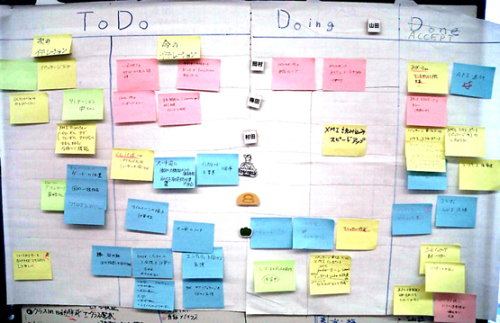
\includegraphics[width=.45\textwidth]{img/scrum-taskboard.jpg}
			\caption{SCRUM Taskboard}
		\end{figure}
		\begin{figure}
			\centering
			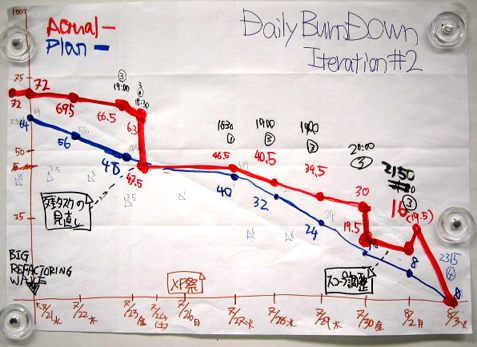
\includegraphics[width=.45\textwidth]{img/scrum-burndown-chart.jpg}
			\caption{SCRUM Burndown Chart}
		\end{figure}
	\end{multicols}
\end{tframe}

\subsection{Rational Unified Process}
\begin{tframe}

\end{tframe}

% ===== real-life examples =========================================================
\section{The HOW (part 2): real-life examples}

\subsection{at Hochschulrechenzentrum, TU Darmstadt}
\begin{tframe}

\end{tframe}

\subsection{at dimetis GmbH}
\begin{tframe}

\end{tframe}

\subsection{at BASF IT-Services}
\begin{tframe}

\end{tframe}

% ===== appendix: bibliography =====================================================
\appendix
\begin{frame}{Bibliography}
	\bibliographystyle{alphanum}
	\bibliography{cmmi-monitoring}
\end{frame}

\end{document}